
%TeXstudio produce a LOT of warning yet still compile.

\documentclass[11pt]{beamer} 

\usetheme{metropolis} %https://github.com/matze/mtheme
\metroset{everytitleformat = regular,progressbar=foot} %settings
\mode<presentation>
%\usecolortheme{dove} %dove
% albatross, beaver, beetle, crane, default, dolphin, dove, orchid, rose, seagull, seahorse, whale, wolverine
%dont use  fly, lily,
%http://mirror.ox.ac.uk/sites/ctan.org/macros/latex/contrib/beamer/doc/beameruserguide.pdf
\setbeamercolor{title separator}{fg = UniBlue}
\setbeamercolor{frametitle}{fg = deepBlue, bg=aBlue!70}

\usepackage{booktabs}
\usepackage[scale=2]{ccicons}
\usepackage{pgfplots}
\usepgfplotslibrary{dateplot}
%\usepackage[demo]{graphicx}
\usepackage[font={small,it}]{caption}
\usepackage{subcaption} %throws a lot of errors but compile

%%LOGO
\usepackage{tikz}
\addtobeamertemplate{frametitle}{}{%
\begin{tikzpicture}[remember picture,overlay]
\node[anchor=north east,yshift=2pt] at (current page.north east) {
\includegraphics[height=0.8cm]{./../logo.png}};
\end{tikzpicture}}

%My std preamble for the docs
%\selectlanguage{british}%
\usepackage[british]{babel}
\usepackage{microtype} %better text
\IfFileExists{lmodern.sty}{\usepackage{lmodern}}{} %type 1 vector font
%
\usepackage{lettrine}
\usepackage{listings} %Add list support
\usepackage{colortbl} %colors in TABLES
%\usepackage{tikz,amsmath, amssymb,bm,color}
\usepackage{nicefrac}
\usepackage{lastpage} %get last page

%COLORS
\usepackage{color}
\definecolor{lightgray}{gray}{0.8} %for colortbl
\definecolor{UniBlue}{RGB}{83,121,170}
\definecolor{deepBlue}{HTML}{000066}
\definecolor{blueBgd}{HTML}{99C8FF}
\definecolor{aBlue}{HTML}{1879F7}

%%%%%%%%%%%%%%%%%%%%%%%%%%%%%%%%%%%%%%%%%%%%%%%%%%%%%%%%%%%%%%%%%%
%FOOTNOTES
%nice look after http://www.dedoimedo.com


%%%%%%%%%%%%%%%%%%%%%%%%%%%%%%%%%%%%%%%%%%%%%%%%%%%%%%%%%%%%%%%%%%%
%TABLE SETTINGS
\usepackage{colortbl} %colors in table
\usepackage{rotating} %rotatins within tables
\usepackage{multirow}
\renewcommand{\arraystretch}{1.2} %add padding/spacing
%\usepackage{adjustbox}%rotating and fitting into page
%

\usepackage{booktabs} % To thicken table lines
%define thickness of table lines
\let\mytoprule\toprule
\renewcommand{\toprule}{\mytoprule[0.20em]}
\let\mytoprule\bottomrule
\renewcommand{\bottomrule}{\mytoprule[0.20em]}
\let\mytoprule\midrule
\renewcommand{\midrule}{\mytoprule[0.08em]}

\usepackage{spreadtab} % for simple calculations

%vertically and horizontally centered multicolumn cells with a fixed width. M{width}
%\newcolumntype{M}[1]{>{\centering\hspace{0pt}}m{#1}}
% each spanned cell has the same width. S{width of multicolumn cell}{number of spanned columns}
%\newcolumntype{S}[2]{>{\centering\hspace{0pt}}m{(#1+(2\tabcolsep+\arrayrulewidth)*(1-#2))/#2}}

%%%%%%%%%%%%%%%%%%%%%%%%%%%%%%%%%%%%%%%%%%%%%%%%%%%%%%%%%%%%%%%%%%%
%TikZ
\usepackage{tikz}

\colorlet{red}{red!50}
\colorlet{green}{green!50}
\colorlet{blue}{blue!50}
\definecolor{yellow}{HTML}{FFFF00}
\colorlet{yellow}{yellow!50}
\definecolor{fiolet}{HTML}{7030A0}
\colorlet{fiolet}{fiolet!50}
\colorlet{bgd_main}{black!50}
\colorlet{bgd}{bgd_main!75}
\colorlet{bgd2}{bgd_main!50}
\colorlet{bgd3}{bgd_main!25}
\colorlet{bgd4}{bgd_main!15}

\usetikzlibrary{shapes,arrows,calc,positioning}

%%%%%%%%%%%%%%%%%%%%%%%%%%%%%%%%%%%%%%%%%%%%%%%%%%%%%%%%%%%%%%%%%%%
% Footnotes in Figs
%\rule[raise-height]{width}{thickness}
\newcommand*{\FigFootnote}[1]{
\noindent \begin{flushleft}
\rule[0.2ex]{0.4\columnwidth}{0.5pt}
\par
\footnotesize
#1
\footnotesize
\end{flushleft}
}

%%%%%%%%%%%%%%%%%%%%%%%%%%%%%%%%%%%%%%%%%%%%%%%%%%%%%%%%%%%%%%%%%%%
%MATH, number display
%need to install siunitx, l3kernel,l3packages
\usepackage{siunitx} %this is for units display

\sisetup{per-mode=fraction, tight-spacing = true , fraction-function = \nicefrac, quotient-mode = fraction}% %nicefrac \tfrac
\sisetup{inter-unit-product = \ensuremath { { } \cdot { } } , exponent-product = \cdot }%
\sisetup{input-product=x , output-quotient =  \ensuremath { { } \times{}}} %for 1x2x3
%number grouping(3), std==true %\sisetup{group-digits = decimal} 
\sisetup{group-minimum-digits = 4} %start grouping from 4 digits, in 3 no groups
\sisetup{range-units = single,range-phrase = \,--\,} %2-3C not 2C-3C %, range-phrase = --
\sisetup{separate-uncertainty=true} %2+-1 not 2(1)
\sisetup{prefixes-as-symbols=true } % , scientific-notation = engineering false for 10^-9 ect ect , exp in multiple of 3
\sisetup{range-phrase = \,-\, } % , refo of ranges
%\sisetup{zero-decimal-to-integer, round-mode = places,round-precision = 3}
%\sisetup{add-arc-degree-zero=true , add-arc-minute-zero=true ,add-arc-second-zero=true} %for angle settings

%This is to auto convert ns,ms,us to 10^-xx s
\DeclareSIUnit[scientific-notation = engineering, prefixes-as-symbols=false]{\psec}{\pico\second}
\DeclareSIUnit[scientific-notation = engineering, prefixes-as-symbols=false]{\nsec}{\nano\second} 
\DeclareSIUnit[scientific-notation = engineering, prefixes-as-symbols=false]{\usec}{\micro\second}
\DeclareSIUnit[scientific-notation = engineering, prefixes-as-symbols=false]{\msec}{\milli\second} 

%...AND SOME UNITS
\DeclareSIUnit\dBm{dBm}
\DeclareSIUnit\ppm{ppm} %{\num{1e-6}}%{ppm}
\DeclareSIUnit\yr{yr} %{{361}\day}<-nice nice
\DeclareSIUnit\cy{cycle} %phase cycle
\DeclareSIUnit\epoch{epoch} %GPS/LL epoch
\DeclareSIUnit\inch{"} %inch 
\DeclareSIUnit\wk{week} %week
\DeclareSIUnit\hr{hrs} %hours
\DeclareSIUnit\min{minute} %hours
\DeclareSIUnit\mile{mi}
\DeclareSIUnit\Mcps{Mcps}
\DeclareSIUnit\bit{bit}
\DeclareSIUnit\chip{chip length}
%Other units
\newcommand*{\GBP}[1]{$\SI{#1}[\textsterling]{}$}


%%%%%SHORTHANDS (Standard Sentences)
%\newcommand*{\Myrange}[3]{$\textrm{\SIrange{#1}{#2}{#3}}$}


%how much work per week
\newcommand*{\wkWrk}[1]{$\SI{#1}{\hr\per\wk}$}

%references
\newcommand*{\tabref}[1]{shown in table \ref{#1} on page \pageref{#1}\xspace}
\newcommand*{\vref}[1]{\ref{#1} on page \pageref{#1}\xspace}


%\renewcommand{\baselinestretch}{1.2} %line spacing
%{\setstretch{1.0}\color{blue} text bla bla } for section strech
\renewcommand{\footnotesize}{\scriptsize} %change footnote sizes
\newcommand{\MatlabRef}{\footnote{History of changes at \url{https://github.com/DfAC/TEQCSPEC}.}}
\newcommand{\thisDocRef}{\footnote{History of changes at \url{https://github.com/DfAC/TeachingSlides/}.}}
%\usepackage{lipsum} % for dummy text only

%Grey text
\definecolor{shadecolor}{RGB}{190,190,190}
%\textcolor{shadecolor}{	\item[Ogaja\_Matlab.7z] Matlab script. To be placed on-line after week2.}


%%%%%%%%%%%%%%%%%%%%%%%%%%%%%%%%%%%%%%%%%%%%%%%%%%%%%%%%%%%%%%%%%%%%%%%%%%%%%%
%%%%%%%%%%%%%%%%%%%%%%%%%%%%%%%%%%%%%%%%%%%%%%%%%%%%%%%%%%%%%%%%%%%%%%%%%%%%%%

\title[H24VLP]{H24VLP Project 1}
\subtitle{Environmental impact on \\the GNSS positioning performance}

\author{LKB}
\institute{NGI}
\date{\today}

\begin{document}
	
	\begin{frame}
		\titlepage
	\end{frame}
	
	% Uncomment these lines for an automatically generated outline.
	\begin{frame}{Outline}
		\tableofcontents
	\end{frame}
	
\section{Introduction}

	\begin{frame}[allowframebreaks]{Project Introduction}
		Aim of the project is to understand the impact of the environment on positioning performance. You will study 
		\begin{itemize}
			\item Positioning performance;
			\item Number of satellites and Signal strength;
			\item Multipath;
		\end{itemize}
		using data collected in three distinctive environments
		\begin{itemize}
			\item Open area;
			\item Foliage (trees);
			\item heavy multipath - between two buildings.
		\end{itemize}
		For the study we expect you to use:
		\begin{itemize}
			\item TEQC command line software;
			\item TEQCSPEC Matlab script visualising multipath;
			\item WangSEU VC++ software;
		\end{itemize}

	\end{frame}

	\begin{frame}{Workflow}
		I suggest following workflow for your analysis:
		
		\begin{itemize}
			\item Extract QC characteristics from RINEX data using \textit{ teqc +qc +plot data.16o};
			\item Use Matlab script for initial visualisation of results;
			%\item \textcolor{shadecolor}{Examine relevant files and teqc summary file};
			\item Use software to output relevant data into CSV file;
			\item Use Matlab script for initial visualisation of results;
			\item \textbf{Analyse data and draw conclusions.}
			\item \alert{Prepare and present a story about your findings.}
		\end{itemize}
	\end{frame}


\section{Software}

	\begin{frame}{TEQC}
		TEQC\footnote{\url{http://www.unavco.org/software/data-processing/TEQC/TEQC.html}. Latest binaries at at bottom of page.} allows translation, editing and quality control of collected GNSS data\footnote{Tutorials are available at \url{http://www.unavco.org/software/data-processing/TEQC/doc/UNAVCO_TEQC_Tutorial.pdf}}. \\
		\medskip
		For example \alert{\textit{ teqc +qc +plot data.16o}} will produce all outputs needed for Matlab script. Use binaries provided with Matlab script as recent ones use non-compatible COMPACT3 format \footnote{\url{http://postal.unavco.org/pipermail/teqc/2013/001594.html}}. Other examples are available in \textit{TEQC\_intro.pdf} introductory document by Sean Ince.

	\end{frame}



	\begin{frame}{TEQCSPEC}
		This matlab script visualise \textit{teqc qc data} using COMPACT2 files created by TEQC. We expect that you will utilise script to identify satellites to analyse. To create plots:
		\begin{itemize}
			\item run \textit{main.m} (F5) selecting script folder as active;
			\item select requested teqc COMPACT2 files;
			\item plots 5-6 visualise multipath on skyplot;
			\item \textcolor{shadecolor}{explore other plots;}
			\item save plots.
		\end{itemize}

		Further description is available in \textit{2006\_Ogaja.pdf}, available, with scripts, at H24VLP Moodle website\MatlabRef.
	\end{frame}	

	\begin{frame}[allowframebreaks]{WangSEU}

	WangSEU is a software created by Denghui Wang, \textit{visiting PhD student from Southeast University, Nanjing, China}. You will use it to output relevant characteristics from RINEX\footnote{you need RINEX 2.11 \textit{*.??o, *.??p *.??n} files.}. Software outputs separate CSV file for each satellite\footnote{Note that $SV_{GLONASS} =  SV_{ID} + 60$ to differentiate from GPS. For example SV64 is GLONASS 4 while SV4 is GPS 4.} with the following columns:\\

	\resizebox{\textwidth}{!}{%fit to page
		\begin{tabular}{cccccccccc} %{l|c|c|c|c}
			%\toprule %\rowcolor{lightgray}
			Epoch[s] & GPS week [s] & SV ID & Elev[deg] & Az[deg] &  MP1 & MP2 & SN1 & SN2 &  SV lock [s] \\
			%\midrule
		\end{tabular}%
	} %resizebox{}

To produce CSV output:
 
\begin{itemize}
	\item start \textit{WangSEU.exe}
	\item from top menu select \textit{Read Rinex File $\rightarrow$ Read single station RINEX file}
\end{itemize}

	\begin{exampleblock}{Example output}{
{\tiny
Epoch,1,GPSSecond,305969,Sat, 10,Ele, 69.46,Azi,147.97,MP1,-13.4718,MP2,-23.1764,SN1,50.25,SN2,45.40,Num,1,\\
Epoch,2,GPSSecond,305970,Sat, 10,Ele, 69.45,Azi,147.97,MP1,-13.4753,MP2,-23.1607,SN1,50.30,SN2,45.15,Num,2,\\
Epoch,3,GPSSecond,305971,Sat, 10,Ele, 69.44,Azi,147.97,MP1,-13.4779,MP2,-23.1643,SN1,50.40,SN2,45.35,Num,3,\\
Epoch,4,GPSSecond,305972,Sat, 10,Ele, 69.43,Azi,147.96,MP1,-13.4686,MP2,-23.1767,SN1,50.45,SN2,45.35,Num,4,\\
} %end of text
		} %end of block
	\end{exampleblock}
	\end{frame}


%changing settings for this area
{\sisetup{round-mode = places,round-precision = 3} 

\begin{frame}{Point coordinates (truth)}
	\begin{table}
		\centering
		\begin{minipage}[t]{\textwidth}%
			\resizebox{\columnwidth}{!}{%
				\begin{tabular}{lcccc} %{l|c|c|c|c}
					\toprule %\rowcolor{lightgray}
					ID & $E[m]$ & $N[m]$ & Ht Ort [m]\footnote{Geoid undulation is \num{48.523}m} & Notes \\
					\midrule
					JUB7 & \num{454729.5517} & \num{339338.9003} & \num{28.9802} & Open Area\\
					JUB8 & \num{454682.3444} & \num{339523.0937} & \num{27.8030} & Trees\\
					UrbanA & \num{454853.269} & \num{339696.63} & \num{29.89} & MP area for Group A\\
					UrbanB & \num{454858.511} & \num{339697.517} & \num{29.854} & MP area for Group B\\
				\end{tabular}%
			}
			\caption{OSGB coordinates for the Project 1}
		\end{minipage}
	\end{table}
	
\end{frame}
} %{\sisetup{round-mode = places,round-precision = 3} 



\section{Comparison examples}

	\begin{frame}{Visualisations}
		Following examples have been carried out by PhD students at NGI and show possible visualisations of multipath:
		
		\begin{itemize}
			\item Sample Matlab output using OS data (Jareer Mohammed);
			\item Sample Denghui Wang visualisation;
			\item Sample Jareer Mohammed visualisation;
		\end{itemize}

	\end{frame}



\begin{frame}[allowframebreaks]{Matlab output}
%Monday 12/01/15, MP2
	\begin{figure}
		\centering
		\begin{subfigure}{.5\textwidth}
			\centering
			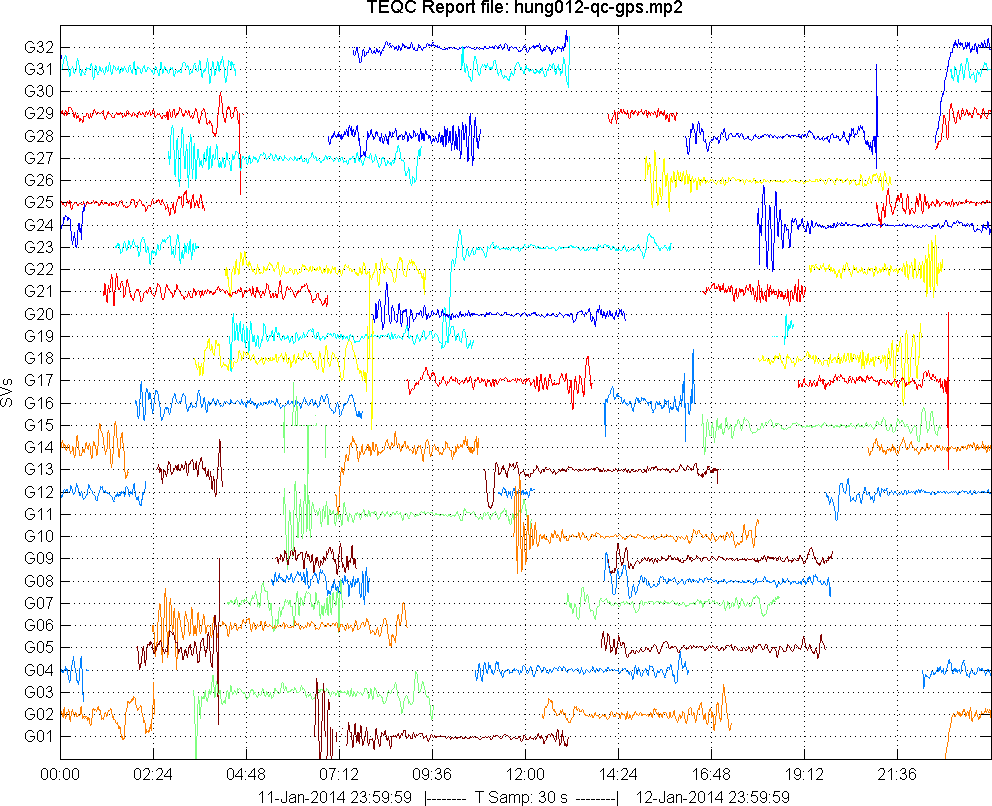
\includegraphics[width=\textwidth]{pic/hung012_qc_gps_mp2.png}
			\caption{HUNG, no MP}
			%\label{fig:sub1}
		\end{subfigure}%
		\begin{subfigure}{.5\textwidth}
			\centering
			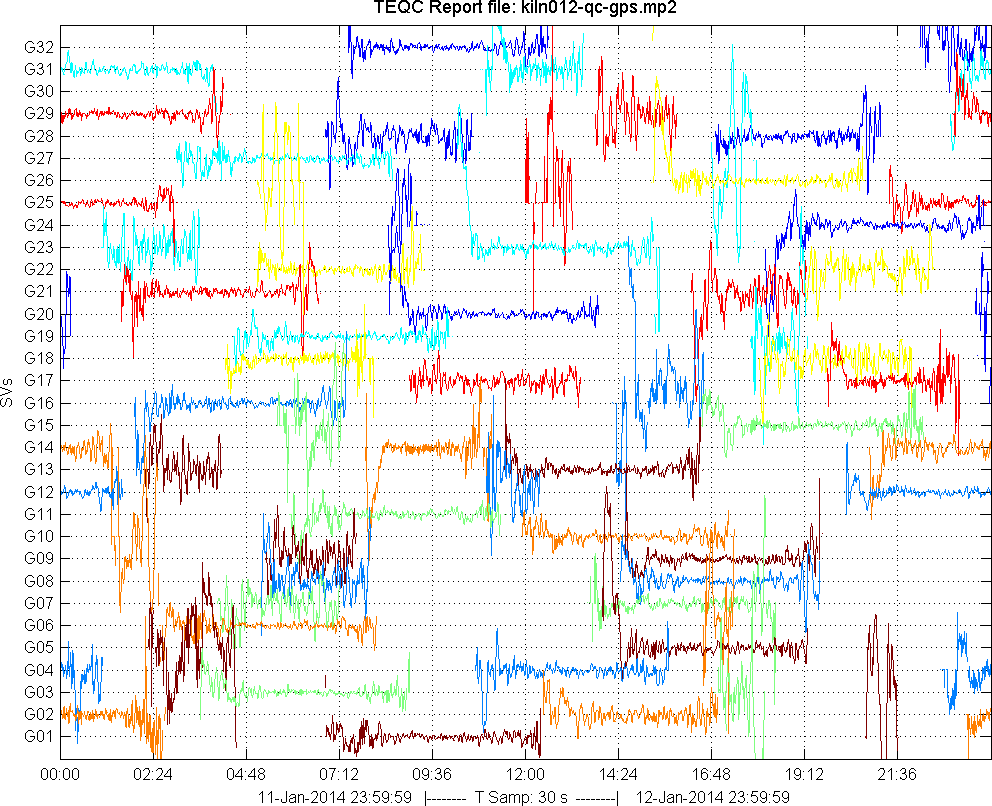
\includegraphics[width=\textwidth]{pic/kiln012_qc_gps_mp2.png}
			\caption{KILN, suspected MP}
			%\label{fig:sub2}
		\end{subfigure}
		\caption{TEQC MP2, day 1}
		% \label{fig:test}
	\end{figure}
%Tuesday 13/01/15, MP2
	\begin{figure}
		\centering
		\begin{subfigure}{.5\textwidth}
			\centering
			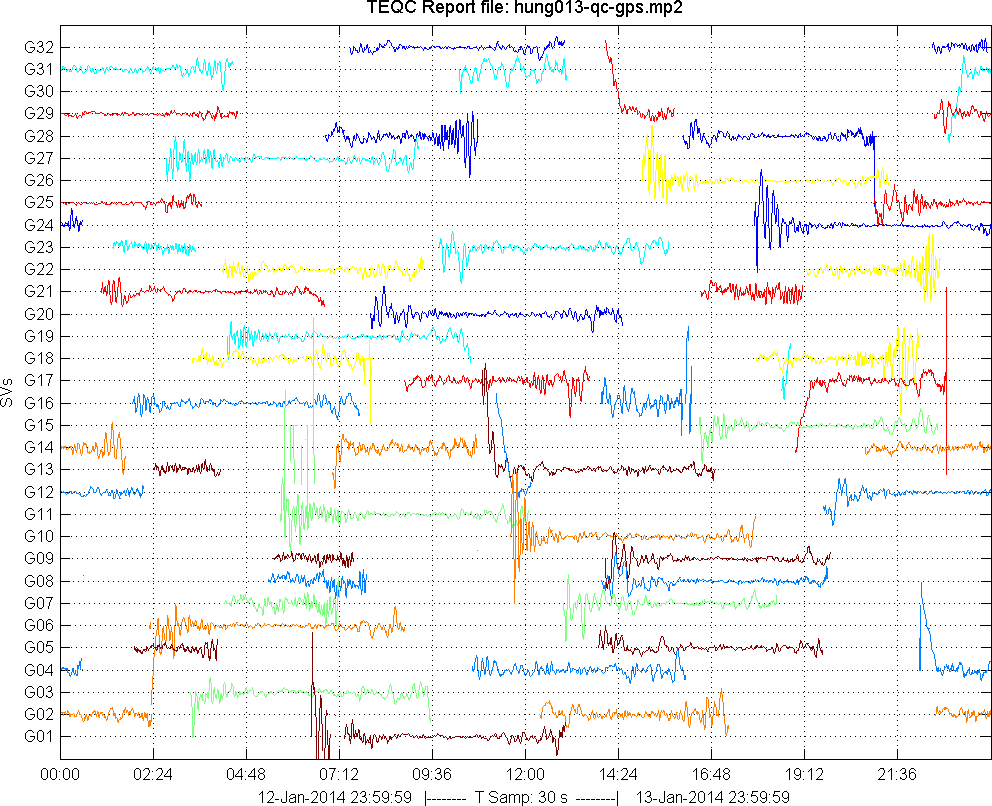
\includegraphics[width=\textwidth]{pic/hung013_qc_gps_mp2.png}
			\caption{HUNG, no MP}
			%\label{fig:sub1}
		\end{subfigure}%
		\begin{subfigure}{.5\textwidth}
			\centering
			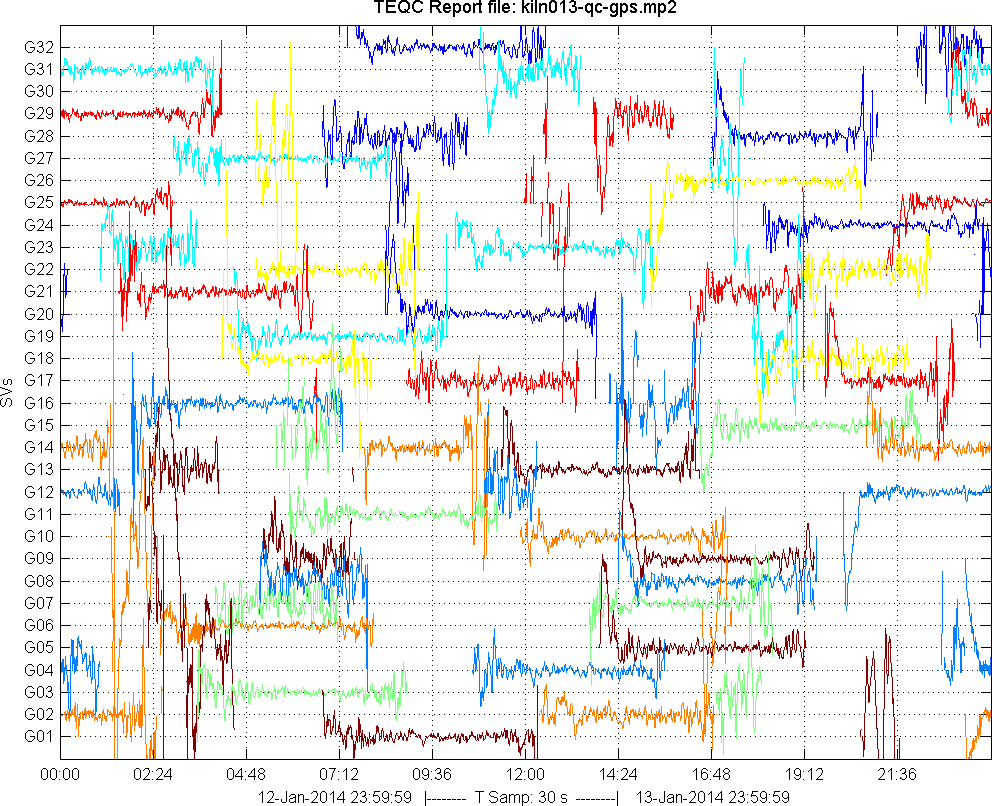
\includegraphics[width=\textwidth]{pic/kiln013_qc_gps_mp2.png}
			\caption{KILN, suspected MP}
			%\label{fig:sub2}
		\end{subfigure}
		\caption{TEQC MP2, day 2}
		% \label{fig:test}
	\end{figure}
\end{frame}



\begin{frame}{Denghui Wang}%{Daily repetition}
	\centering
	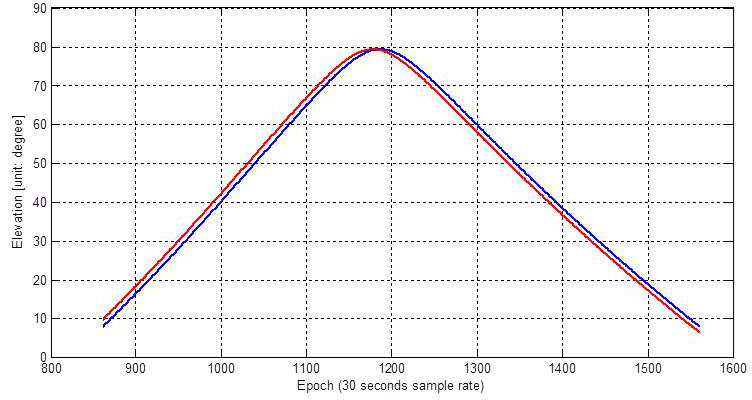
\includegraphics[height=.35\textheight]{pic/DW_reporbits.png}
	\captionof{figure}{Visualisation} %to make images on top of each other
	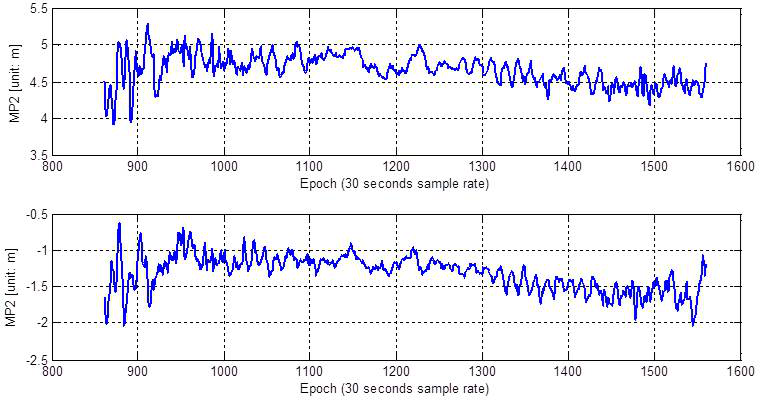
\includegraphics[height=.4\textheight]{pic/DW_mp.png} 
	%\captionof{figure}{Example of visualisation}
\end{frame}

\begin{frame}{Jareer Mohammed}%{Daily repetition}

	\begin{figure}
		\centering
		\begin{subfigure}{.5\textwidth}
			\centering
			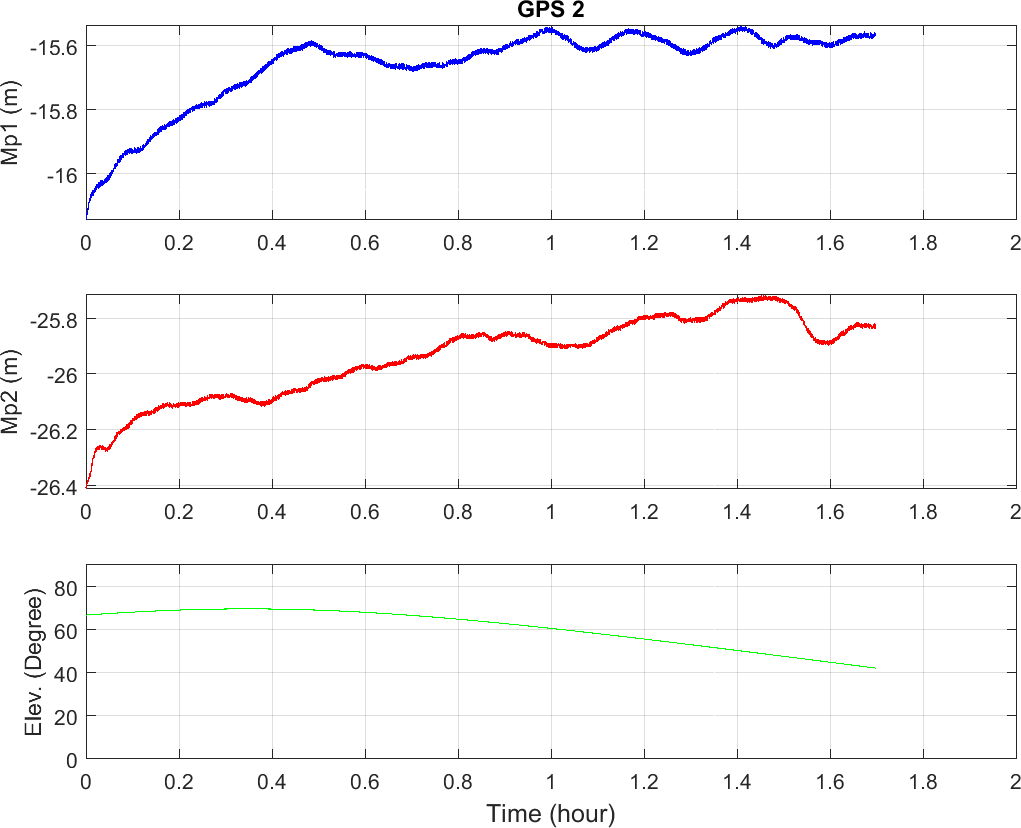
\includegraphics[width=\textwidth]{pic/2_GS10_test_option_12.png}
			\caption{Open sky}
			%\label{fig:sub1}
		\end{subfigure}%
		\begin{subfigure}{.5\textwidth}
			\centering
			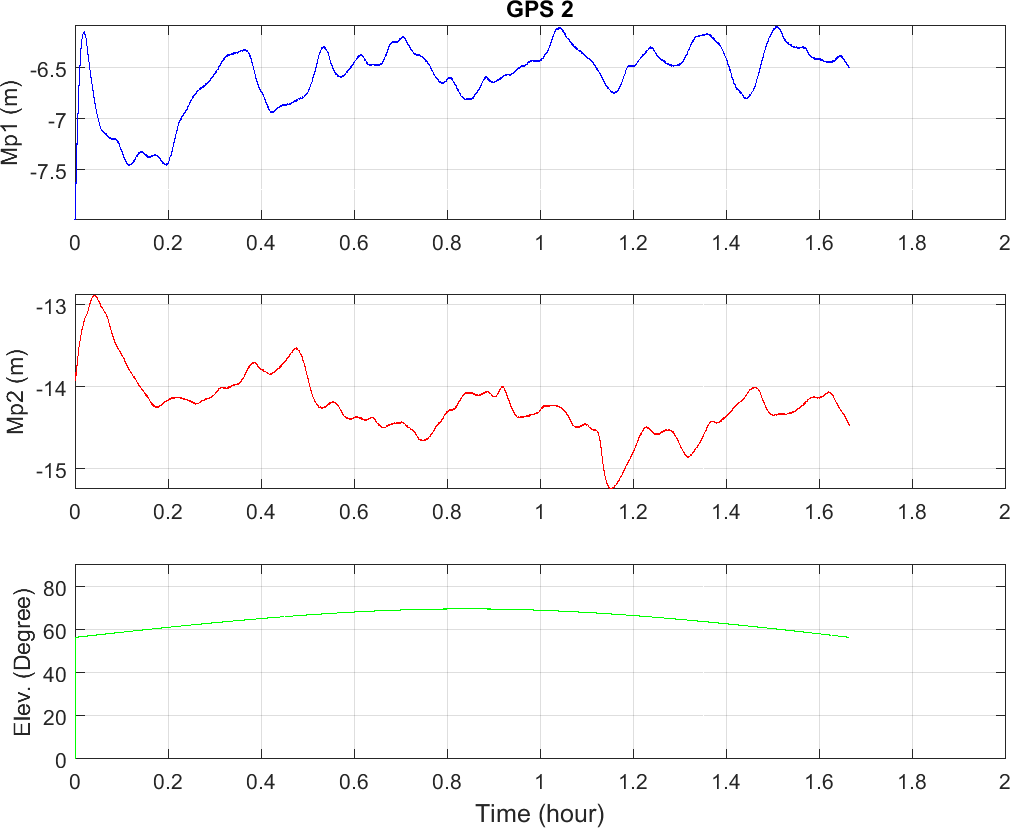
\includegraphics[width=\textwidth]{pic/2_GS09_test_option_12.png}
			\caption{Urban area}
			%\label{fig:sub2}
		\end{subfigure}
		\caption{Comparison for GPS SV2}
		% \label{fig:test}
	\end{figure}
\end{frame}

\section{Summary}


	\begin{frame}{Supporting files}
	You will study the impact of the environment on positioning performance using software provided. We expect you to produce own graphs using outputs from the provided software. Following files can be found on the accompanying Moodle site:

		\begin{description}
		\item[H24VLP\_P1\_MP.pdf] This presentation\thisDocRef;
		\item[TEQC\_intro.pdf] Introduction to TEQC (Sean Ince);
		\item[teqc.zip] Old teqc 64bit Windows binary to produce Matlab script inputs;
		\item[2006\_Ogaja.pdf] Paper describing TEQCSPEC Matlab script;
		\item[Matlab.zip] TEQCSPEC Matlab script\MatlabRef. Use \textit{main.m} to run it;
		\item[WangSEU.zip] VC++ binary producing CSV files from RINEX.
	\end{description}

	%For older versions please refer to the GitHub site.
	\end{frame}


%Final slide
\setbeamercolor{background canvas}{bg=blueBgd!60}
\plain{Good luck}



\end{document}
